%TO DO

%PRIORITY: HIGH         FINISH ALL THE TASKS IN THE COMMENTS
%STYLING ISSUES (ADD TO THE LIST IF THERE IS ONE)
    %PRIORITY: LOW      DIFFICULTY: EASY        CREATE DIFFERENT APPENDIXS
    %PRIORITY: MEDIUM   DIFFICULTY: EASY        @SQL QUERIES SECTION DOESNT HAVE A DESCRIPTION/EXPLANATION OF WHAT THE QUERY DOES (ONE SOLUTION COULD JUST BE LITERALLY CONTINUE ON THE NEXT LINE. A HARDER SOLUTION TO IMPLEMENT WOULD BE DO TWO COLUMNS)
    %PRIORITY: MEDIUM   DIFFICULTY: HARD        DESCRIPTION "BLEEDS OUT" OF SECTION @DIAGRAMS NOT SURE WHY IT DOES THIS...
    %PRIORITY: LOW      DIFFICULTY: EASY        SPELL OUT SUBSECTION @SQL QUERY INSTEAD OF ACRONYM
    %PRIORITY: IDK      DIFFICULTY: IDK         LINE SPACING IS A LITTLE TOO CLOSE IMO
%IF NO ONE HAS ANY ISSUES WITH OUR TEAM NAME WELL KEEP IT (ITS BETTER THAN "TEAM 4" IMO)
%INSERT PAGEBREAKS AS YOU SEE FIT AFTER FINISHING WRITING
%DELETE COMPLETED COMMENTS (CLEANUP)

\documentclass{article}
\usepackage{textcomp}
\usepackage{pdfpages}
\usepackage{bold-extra}
\usepackage{setspace}
\usepackage[section]{placeins}
\usepackage{amssymb,amsthm,latexsym,xcolor,graphicx,hyperref,geometry, array}
\usepackage[fleqn]{amsmath}
\usepackage[shortlabels]{enumitem}
\usepackage{multicol}
\usepackage{relsize}
\usepackage{systeme}
\usepackage{commath}
\usepackage{listings}
\usepackage{enumitem}
\usepackage{tikz}
\usepackage{fancyhdr}
\usepackage{tikz}
\usepackage{pdfpages}
\usetikzlibrary{shapes.geometric, arrows}
\tikzstyle{startstop} = [rectangle, rounded corners, minimum width=3cm, minimum height=1cm,text centered, draw=black, fill=green!30]
\tikzstyle{io} = [trapezium, trapezium left angle=70, trapezium right angle=110, minimum width=3cm, minimum height=1cm, text centered, draw=black, fill=blue!30]
\tikzstyle{process} = [rectangle, minimum width=3cm, minimum height=1cm, text centered, draw=black, fill=cyan!30]
\tikzstyle{process1} = [rectangle, minimum width=3cm, minimum height=1cm, text centered, draw=black, fill=orange!30]
\tikzstyle{process2} = [rectangle, minimum width=3cm, minimum height=1cm, text centered, draw=black, fill=red!30]
\tikzstyle{decision} = [diamond, minimum width=3cm, minimum height=1cm, text centered, draw=black, fill=green!30]
\tikzstyle{arrow} = [thick,->,>=stealth]

\geometry{top=1in,bottom=1in,right=1in,left=1in}
\pagestyle{fancy}
\fancyhf{}
\lhead{\rightmark}
\lfoot{Simple Inventory: Inventory Management Tracking Application by Team 8}
%\lfoot{Project 2: Database by Jun Suk ``Justin" Yoo et al.}
\rfoot{\thepage}
\renewcommand{\headrulewidth}{0.75pt}
%\setlength{\parindent}{4em}
%\setlength{\parskip}{1em}
%\renewcommand{\baselinestretch}{1}

%none of the above work idk
\newcolumntype{P}[1]{>{\centering\arraybackslash}p{#1}}
\lstset
{
	language=c,
	basicstyle=\footnotesize,
	numbers=left,
	stepnumber=1,
	tabsize=1,
	morekeywords={to, downto, and},
	numbersep=0pt,
	literate={\ \ }{{\ }}
}
\usepackage[utf8]{inputenc}

\title{\Huge{\textbf{CSCE-431: Software Engineering}\\\vspace{0.75cm}Inventory Management Tracking Application\\\huge Iteration 0}\\\vspace{1cm}\huge Team 8:  \textit{Simple Inventory}}
\author{ \Large Jireh Ferrer
    \and
        \Large Ryan Parker
    \and
        \Large Sabrina Smith
    \and
        \Large Hanson Yu }
\date{ \vspace{1cm} \large 2021 December 30 }

\begin{document}
%\maketitle%
\thispagestyle{empty}
\maketitle
\setcounter{secnumdepth}{0}

\thispagestyle{empty}
\pagebreak
\tableofcontents
\thispagestyle{empty}
\pagebreak
\thispagestyle{fancy}
%\renewcommand{\sectionmark}[1]{\markright{\thesection.\ #1}}%
\renewcommand{\sectionmark}[1]{\markright{#1}{}}
\setcounter{page}{1}
    \section{Team}
        \subsection{Name Branding and Logo}
            Our team's name is the same as our product's name: \textit{Simple Inventory}.
            \begin{figure}[!htb]
                \quad\quad\quad\quad\quad\quad\quad\quad\quad\quad\quad\quad\quad\quad\quad\quad\quad\quad\quad
\includegraphics[scale=0.15]{resources/keyboard_key_i.png}
                \caption{\textit{Simple Inventory} Logo}
                \label{fig:Diagram 3}
            \end{figure}
            
            \noindent We will be investing more time into our branding and logo design later.\\
            
        \subsection{Roles}
        \begin{center}
            \Large \textbf{\textit{Simple Inventory}}
        \end{center}
        \begin{center}
            \begin{tabular}{ P{3cm}|P{3cm} } 
                 \\
                 \large \textbf{Role} & \large \textbf{Name} \\
                 \\
                 \\
                 Scrum Master & Hanson Yu \\
                 \\
                 \\
                 Product Owner & Sabrina Smith \\
                 \\
                 \\
                 Software Engineer Developer & Jireh Ferrer\linebreak Ryan Parker\linebreak Sabrina Smith\linebreak Hanson Yu \\ 
            \end{tabular}
        \end{center}
        
\pagebreak

    \section{Customer Meeting Details and Notes}
        \subsection{Date Time and Place}
            Originally our first meeting with the customers (Phillip Ritchey and Robert Lightfoot) was scheduled by the Product Owner to be on the 29th of December 2021. However due to time constraints the meeting was later moved to the morning of the 30th of December 2021. At approximately 10:53 Eastern European Standard Time (GMT+2), in an initial meeting with the customers that lasted around half an hour at the Thessaloniki YMCA (Nik. Germanou 1, Thessaloniki 546 21), the Simple Inventory Team discussed project and application requirements with the customers.
            
         \subsection{Summary}
                Developing and maintaining a database system with an easy to use user interface can be costly and cumbersome. Our main customer’s need is that they need a simple and responsive inventory management tracker that can help them conduct their business by keeping track of their products. Examples of target customers include libraries to manage their books, student recreation centers to manage their equipment, etc.\\

                \noindent Our application currently is designed to be generic enough to meet all the varied customer needs through supporting the most basic functionality for creating and deleting items from the inventory management system and adding and removing quantities of those items. Administrators and other users of the system such as workers and employees will be able to intuitively use this application to more efficiently carry out their everyday tasks.    
            
        \subsection{Meeting Notes}
            Feature ideas:
            \begin{itemize}
                \item[-] API for adding and checking inventory
                \item[-] Consumables vs constants
                \item[-] Cost of replacement base on acquisition date
                \item[-] Admin can add and update products/quantities
                \item[-] Users can checkout items
                \item[-] Usage history of items in inventory
                \item[-] Design for extendibility
                \item[-] Reservations
                \item[-] Report generation
                \item[-] Predictive usage based on past usage and current inventory
            \end{itemize}
            
            \noindent Potential use cases:
            \begin{itemize}
                \item[-] Library checkout
                \item[-] Rec center equipment checkout
                \item[-] Tool shed tools checkout and fertilizer/consumables
                \item[-] Wine
                \item[-] T shirts
                \item[-] Washer/dryer availability
                \item[-] Parking garage/parking spot availability
                \item[-] Talk to student marketplace team about project synergy and subleasing team
            \end{itemize}
            
\pagebreak
    
    \section{User Stories}
        \subsection{User Story 1}
            \texttt{Feature: Add a new item to an inventory}\\
            \texttt{\phantom{\quad} As an administrator}\\
            \texttt{\phantom{\quad} So that I can track a new item}\\
            \texttt{\phantom{\quad} I want to be able to add an item to the inventory database}
        \subsection{User Story 2}
            \texttt{Feature: Increase quantity of an item}\\
            \texttt{\phantom{\quad} As a user}\\
            \texttt{\phantom{\quad} So that I can manage new stock arrival to inventory}\\
            \texttt{\phantom{\quad} I want to be able to increase the quantity of a specific item in the inventory}
        \subsection{User Story 3}
            \texttt{Feature: Decrease quantity of an item}\\
            \texttt{\phantom{\quad} As a user}\\
            \texttt{\phantom{\quad} So that I can manage reduction of inventory}\\
            \texttt{\phantom{\quad} I want to be able to decrease the quantity of a specific item in the inventory}
        \subsection{User Story 4}
            \texttt{Feature: Remove an existing item from an inventory}\\
            \texttt{\phantom{\quad} As an administrator}\\
            \texttt{\phantom{\quad} So that I can keep relevant items in inventory}\\
            \texttt{\phantom{\quad} I want to be able to remove an item from the inventory database}
            
\pagebreak

    \section{User Interface}
        \subsection{UI Mockup Storyboard}
            Below is a rough draft scan of the sketches that were made for a lo-fi UI Mockup and storyboard for the 4 user stories that are outlined in the User Stories section.\\
            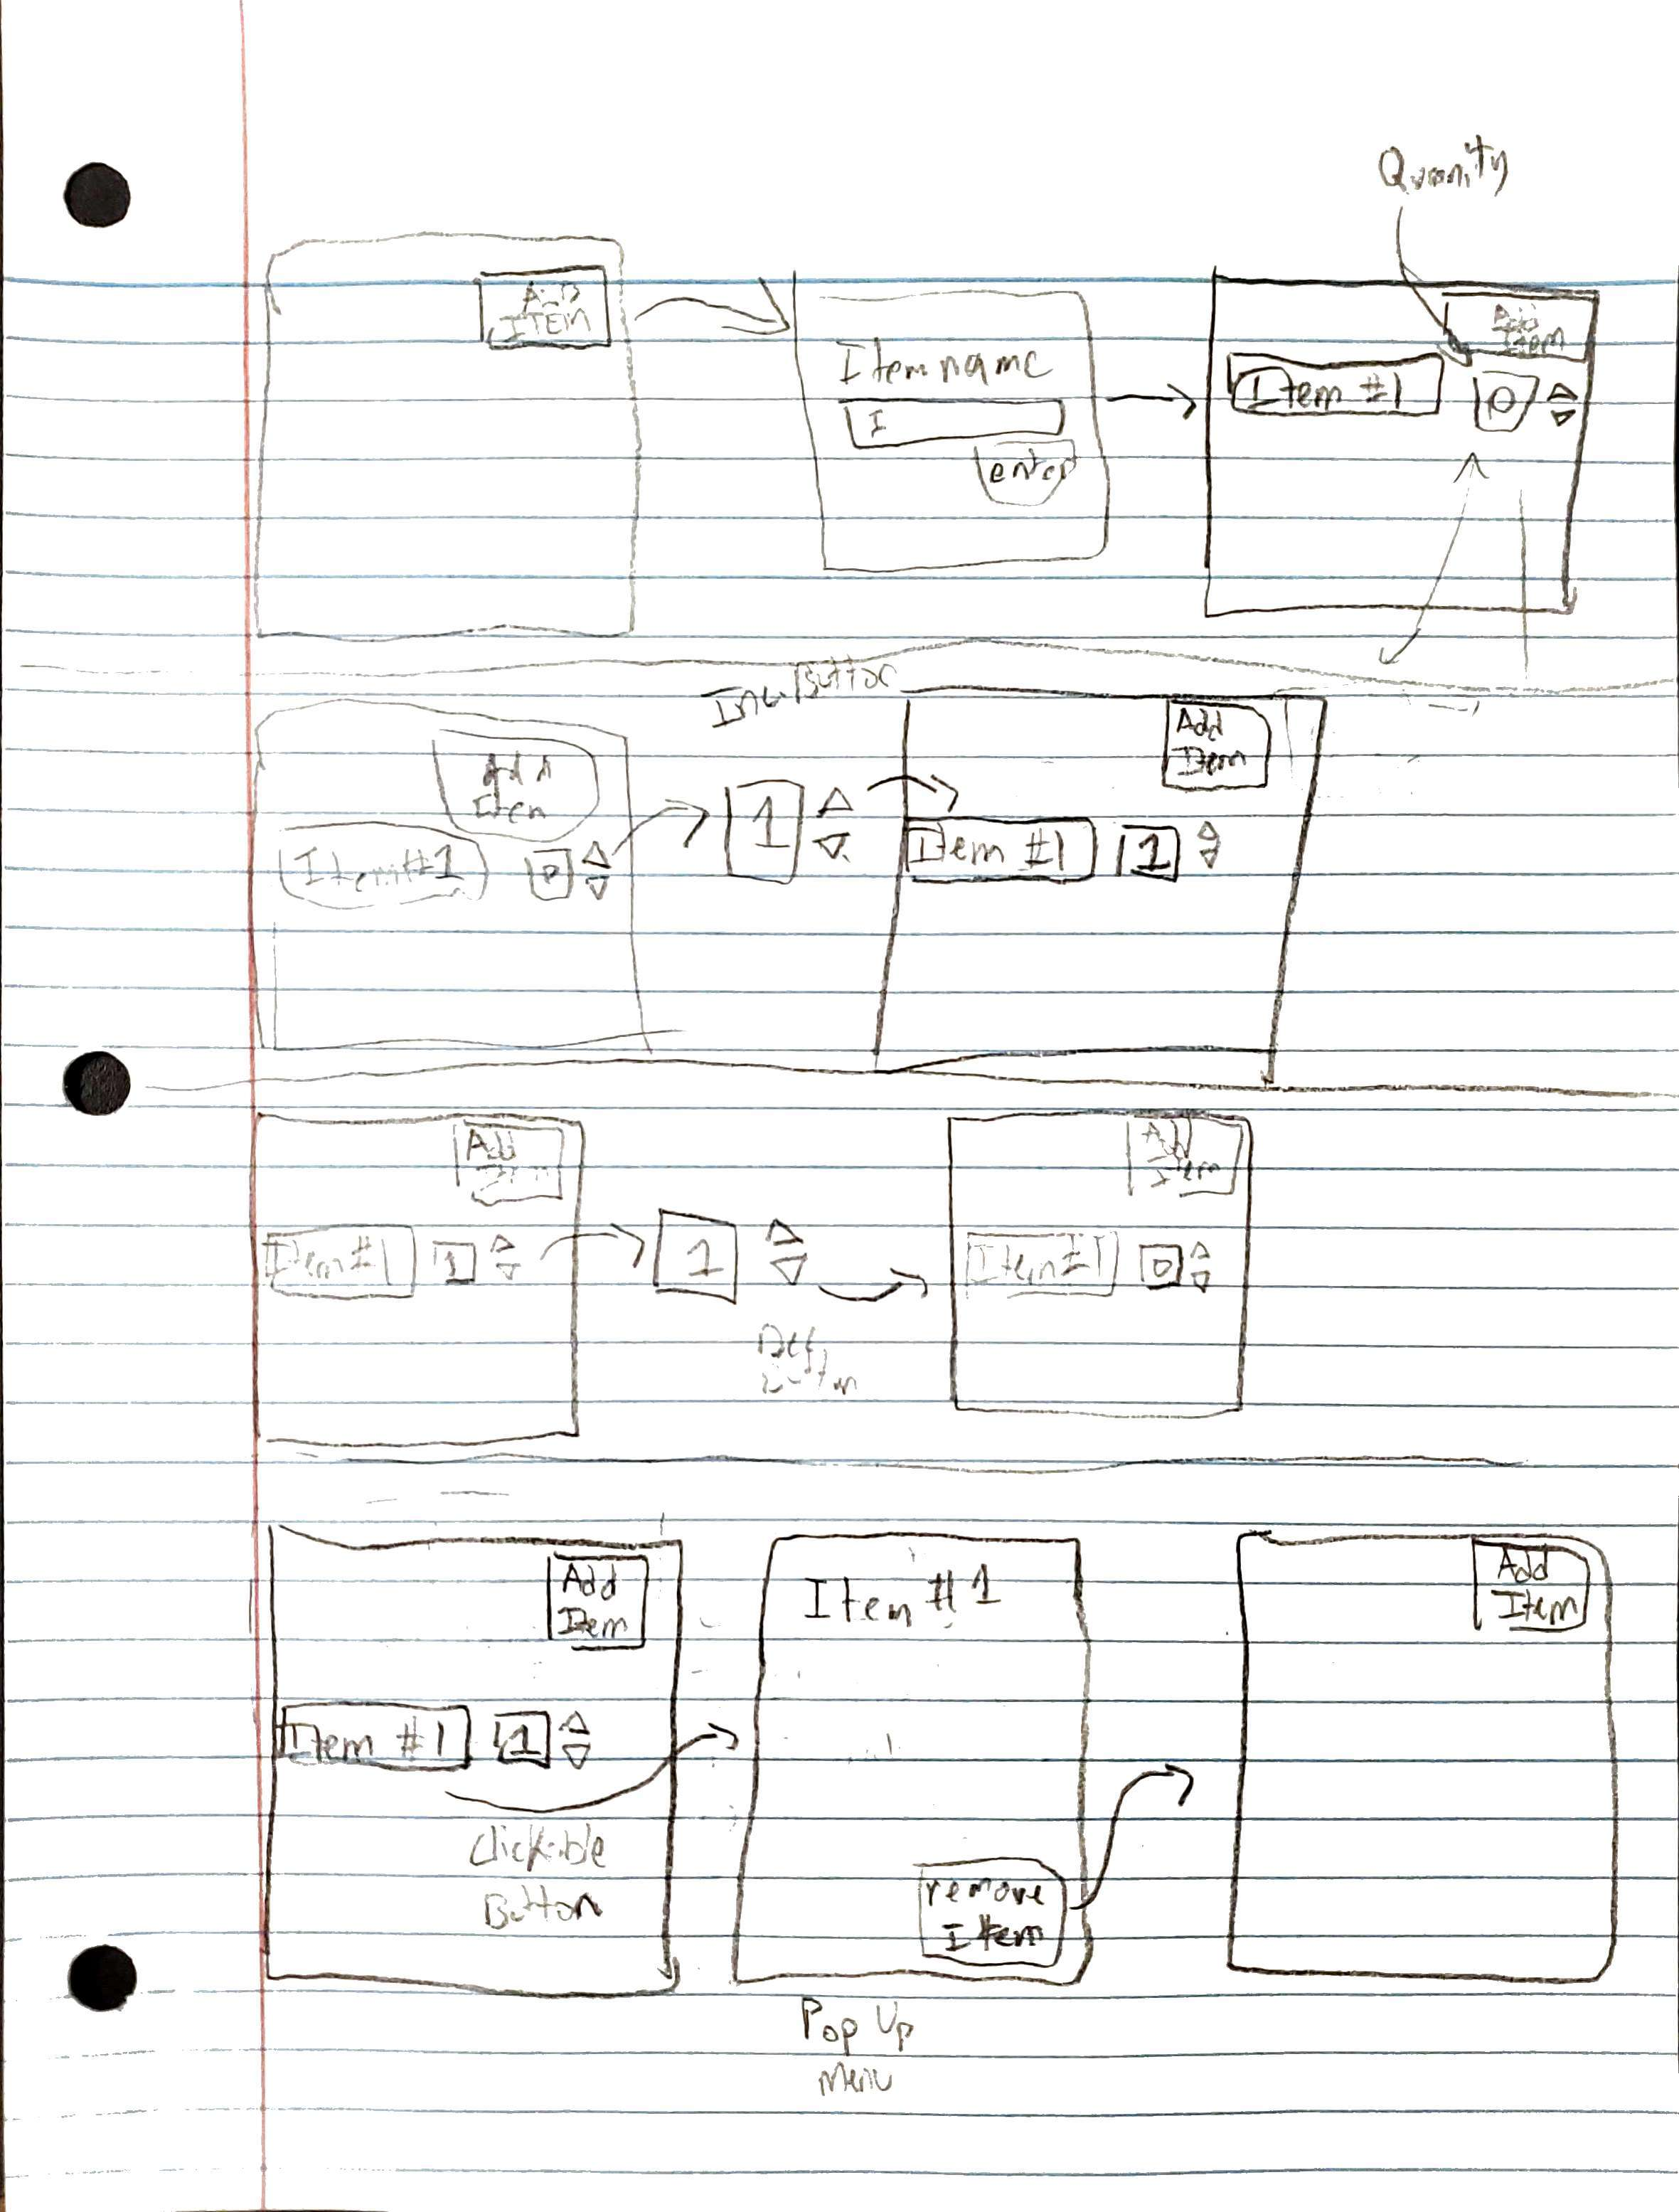
\includegraphics[scale=0.18]{resources/storyboard.jpg}
        \subsection{Diagrammed User Interface}
            

\tikzset{every picture/.style={line width=0.75pt}} %set default line width to 0.75pt        

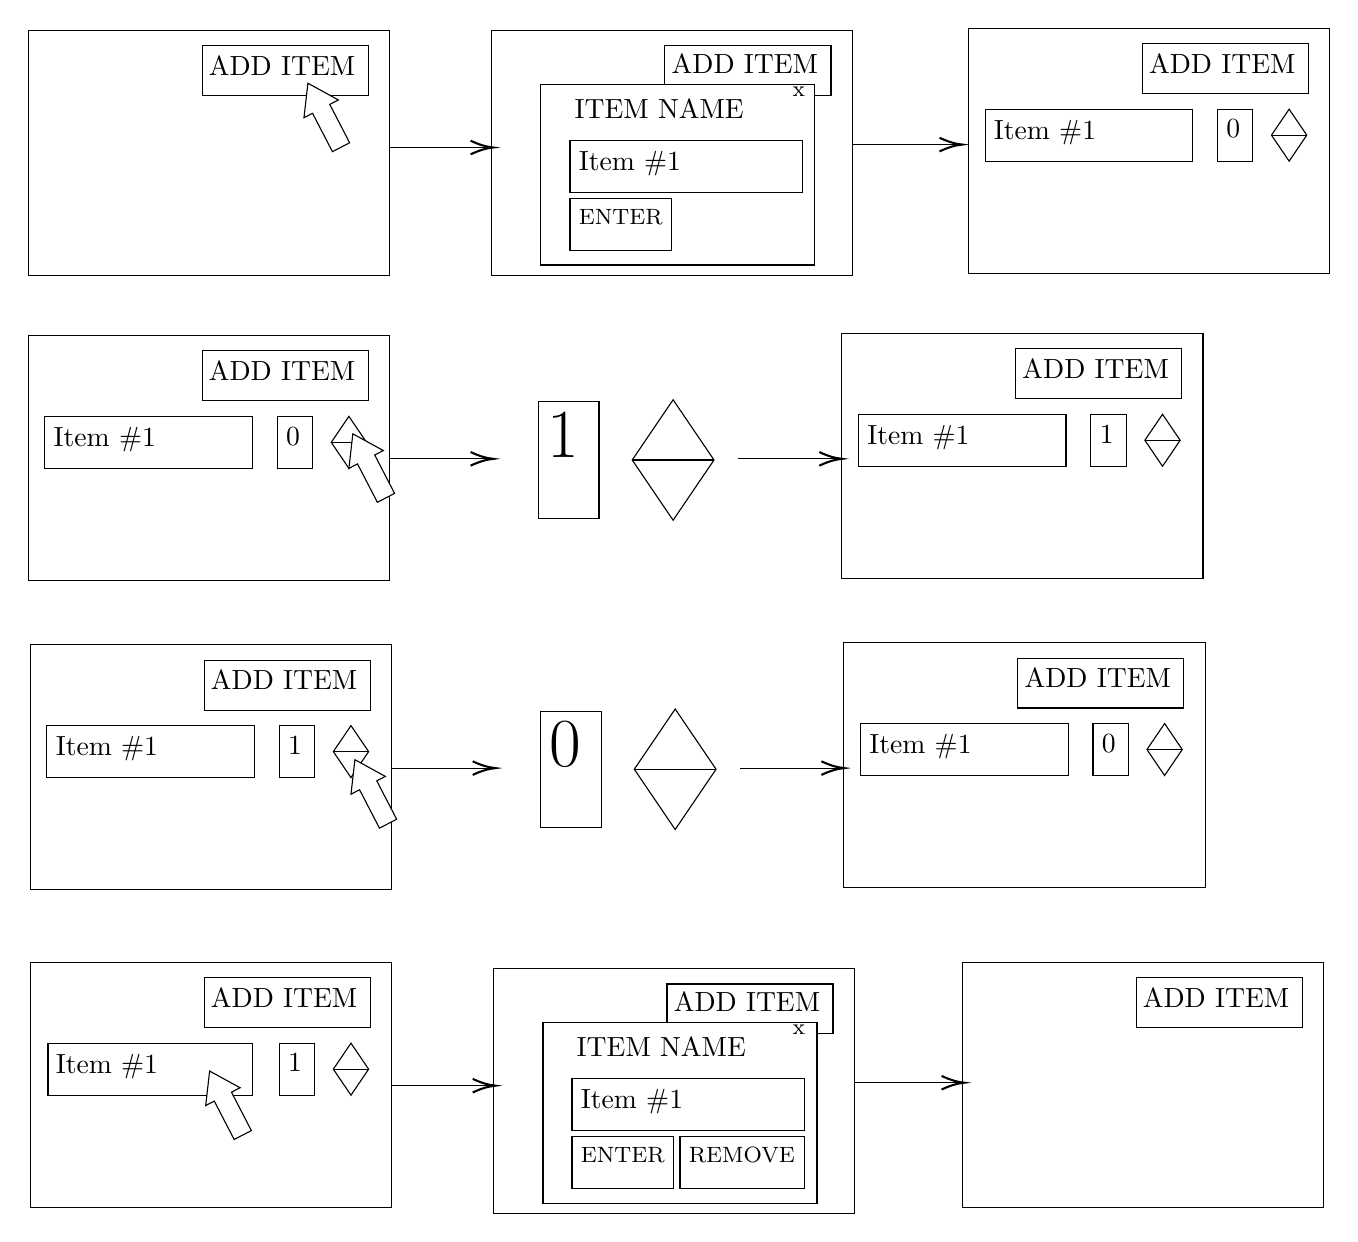
\begin{tikzpicture}[x=0.75pt,y=0.75pt,yscale=-1,xscale=1]
%uncomment if require: \path (0,974); %set diagram left start at 0, and has height of 974

%Shape: Rectangle [id:dp07251084289175491] 
\draw   (21,47) -- (195,47) -- (195,165.05) -- (21,165.05) -- cycle ;
%Shape: Rectangle [id:dp9176159456698147] 
\draw   (104.75,54.46) -- (184.75,54.46) -- (184.75,78.5) -- (104.75,78.5) -- cycle ;
%Up Arrow [id:dp09675630036719696] 
\draw  [fill={rgb, 255:red, 255; green, 255; blue, 255 }  ,fill opacity=1 ] (153.85,89.12) -- (155.75,72.5) -- (170.42,80.55) -- (166.28,82.69) -- (175.86,101.19) -- (167.57,105.48) -- (157.99,86.98) -- cycle ;
%Shape: Rectangle [id:dp6625279645562838] 
\draw   (474,46) -- (648,46) -- (648,164.05) -- (474,164.05) -- cycle ;
%Shape: Rectangle [id:dp371177110764245] 
\draw   (557.75,53.46) -- (637.75,53.46) -- (637.75,77.5) -- (557.75,77.5) -- cycle ;
%Flowchart: Sort [id:dp8961259135558852] 
\draw   (628.5,85) -- (637,97.52) -- (628.5,110.05) -- (620,97.52) -- cycle ; \draw   (620,97.52) -- (637,97.52) ;
%Shape: Rectangle [id:dp9853128156580513] 
\draw   (21,194) -- (195,194) -- (195,312.05) -- (21,312.05) -- cycle ;
%Shape: Rectangle [id:dp6446569839456215] 
\draw   (104.75,201.46) -- (184.75,201.46) -- (184.75,225.5) -- (104.75,225.5) -- cycle ;
%Flowchart: Sort [id:dp18553810859527253] 
\draw   (175.5,233) -- (184,245.52) -- (175.5,258.05) -- (167,245.52) -- cycle ; \draw   (167,245.52) -- (184,245.52) ;
%Up Arrow [id:dp777452711042915] 
\draw  [fill={rgb, 255:red, 255; green, 255; blue, 255 }  ,fill opacity=1 ] (175.5,258.05) -- (177.4,241.42) -- (192.07,249.47) -- (187.93,251.61) -- (197.51,270.11) -- (189.22,274.4) -- (179.64,255.9) -- cycle ;
%Straight Lines [id:da07782150417371159] 
\draw    (195.07,253.47) -- (243.07,253.47) ;
\draw [shift={(245.07,253.47)}, rotate = 180] [color={rgb, 255:red, 0; green, 0; blue, 0 }  ][line width=0.75]    (10.93,-3.29) .. controls (6.95,-1.4) and (3.31,-0.3) .. (0,0) .. controls (3.31,0.3) and (6.95,1.4) .. (10.93,3.29)   ;
%Flowchart: Sort [id:dp940612138479286] 
\draw   (331.7,225) -- (351.4,254.02) -- (331.7,283.05) -- (312,254.02) -- cycle ; \draw   (312,254.02) -- (351.4,254.02) ;
%Shape: Rectangle [id:dp5391354332231928] 
\draw   (413,193) -- (587,193) -- (587,311.05) -- (413,311.05) -- cycle ;
%Shape: Rectangle [id:dp8140986162188713] 
\draw   (496.75,200.46) -- (576.75,200.46) -- (576.75,224.5) -- (496.75,224.5) -- cycle ;
%Flowchart: Sort [id:dp8819807449569035] 
\draw   (567.5,232) -- (576,244.52) -- (567.5,257.05) -- (559,244.52) -- cycle ; \draw   (559,244.52) -- (576,244.52) ;
%Straight Lines [id:da8987558809198644] 
\draw    (363.07,253.47) -- (411.07,253.47) ;
\draw [shift={(413.07,253.47)}, rotate = 180] [color={rgb, 255:red, 0; green, 0; blue, 0 }  ][line width=0.75]    (10.93,-3.29) .. controls (6.95,-1.4) and (3.31,-0.3) .. (0,0) .. controls (3.31,0.3) and (6.95,1.4) .. (10.93,3.29)   ;
%Shape: Rectangle [id:dp8585433678838914] 
\draw   (22,343) -- (196,343) -- (196,461.05) -- (22,461.05) -- cycle ;
%Shape: Rectangle [id:dp5587420912684615] 
\draw   (105.75,350.46) -- (185.75,350.46) -- (185.75,374.5) -- (105.75,374.5) -- cycle ;
%Flowchart: Sort [id:dp14933364977031172] 
\draw   (176.5,382) -- (185,394.52) -- (176.5,407.05) -- (168,394.52) -- cycle ; \draw   (168,394.52) -- (185,394.52) ;
%Up Arrow [id:dp3366812462989748] 
\draw  [fill={rgb, 255:red, 255; green, 255; blue, 255 }  ,fill opacity=1 ] (176.5,415.05) -- (178.4,398.42) -- (193.07,406.47) -- (188.93,408.61) -- (198.51,427.11) -- (190.22,431.4) -- (180.64,412.9) -- cycle ;
%Straight Lines [id:da07486097660178204] 
\draw    (196.07,402.47) -- (244.07,402.47) ;
\draw [shift={(246.07,402.47)}, rotate = 180] [color={rgb, 255:red, 0; green, 0; blue, 0 }  ][line width=0.75]    (10.93,-3.29) .. controls (6.95,-1.4) and (3.31,-0.3) .. (0,0) .. controls (3.31,0.3) and (6.95,1.4) .. (10.93,3.29)   ;
%Flowchart: Sort [id:dp5455420979745622] 
\draw   (332.7,374) -- (352.4,403.02) -- (332.7,432.05) -- (313,403.02) -- cycle ; \draw   (313,403.02) -- (352.4,403.02) ;
%Shape: Rectangle [id:dp7343311475121899] 
\draw   (414,342) -- (588,342) -- (588,460.05) -- (414,460.05) -- cycle ;
%Shape: Rectangle [id:dp5306204219871282] 
\draw   (497.75,349.46) -- (577.75,349.46) -- (577.75,373.5) -- (497.75,373.5) -- cycle ;
%Flowchart: Sort [id:dp23034549078953903] 
\draw   (568.5,381) -- (577,393.52) -- (568.5,406.05) -- (560,393.52) -- cycle ; \draw   (560,393.52) -- (577,393.52) ;
%Straight Lines [id:da7628023020916785] 
\draw    (364.07,402.47) -- (412.07,402.47) ;
\draw [shift={(414.07,402.47)}, rotate = 180] [color={rgb, 255:red, 0; green, 0; blue, 0 }  ][line width=0.75]    (10.93,-3.29) .. controls (6.95,-1.4) and (3.31,-0.3) .. (0,0) .. controls (3.31,0.3) and (6.95,1.4) .. (10.93,3.29)   ;
%Shape: Rectangle [id:dp25335603039843124] 
\draw   (22,496) -- (196,496) -- (196,614.05) -- (22,614.05) -- cycle ;
%Shape: Rectangle [id:dp5921405615419397] 
\draw   (105.75,503.46) -- (185.75,503.46) -- (185.75,527.5) -- (105.75,527.5) -- cycle ;
%Flowchart: Sort [id:dp5717022740682991] 
\draw   (176.5,535) -- (185,547.52) -- (176.5,560.05) -- (168,547.52) -- cycle ; \draw   (168,547.52) -- (185,547.52) ;
%Straight Lines [id:da17474286834294417] 
\draw    (196.07,555.47) -- (244.07,555.47) ;
\draw [shift={(246.07,555.47)}, rotate = 180] [color={rgb, 255:red, 0; green, 0; blue, 0 }  ][line width=0.75]    (10.93,-3.29) .. controls (6.95,-1.4) and (3.31,-0.3) .. (0,0) .. controls (3.31,0.3) and (6.95,1.4) .. (10.93,3.29)   ;
%Shape: Rectangle [id:dp10887716724097518] 
\draw   (30.5,535.05) -- (129,535.05) -- (129,560.05) -- (30.5,560.05) -- cycle ;
%Up Arrow [id:dp9067301838835973] 
\draw  [fill={rgb, 255:red, 255; green, 255; blue, 255 }  ,fill opacity=1 ] (106.5,565.05) -- (108.4,548.42) -- (123.07,556.47) -- (118.93,558.61) -- (128.51,577.11) -- (120.22,581.4) -- (110.64,562.9) -- cycle ;
%Shape: Rectangle [id:dp35724990607958684] 
\draw   (245,499) -- (419,499) -- (419,617.05) -- (245,617.05) -- cycle ;
%Shape: Rectangle [id:dp982657023427363] 
\draw   (328.75,506.46) -- (408.75,506.46) -- (408.75,530.5) -- (328.75,530.5) -- cycle ;
%Straight Lines [id:da13948267852288643] 
\draw    (419,554.05) -- (470,554.05) ;
\draw [shift={(472,554.05)}, rotate = 180] [color={rgb, 255:red, 0; green, 0; blue, 0 }  ][line width=0.75]    (10.93,-3.29) .. controls (6.95,-1.4) and (3.31,-0.3) .. (0,0) .. controls (3.31,0.3) and (6.95,1.4) .. (10.93,3.29)   ;
%Shape: Rectangle [id:dp4702071698363386] 
\draw  [fill={rgb, 255:red, 255; green, 255; blue, 255 }  ,fill opacity=1 ] (269,525) -- (401,525) -- (401,612.05) -- (269,612.05) -- cycle ;
%Straight Lines [id:da5701773903629208] 
\draw    (195.07,103.47) -- (243.07,103.47) ;
\draw [shift={(245.07,103.47)}, rotate = 180] [color={rgb, 255:red, 0; green, 0; blue, 0 }  ][line width=0.75]    (10.93,-3.29) .. controls (6.95,-1.4) and (3.31,-0.3) .. (0,0) .. controls (3.31,0.3) and (6.95,1.4) .. (10.93,3.29)   ;
%Shape: Rectangle [id:dp8444930567215794] 
\draw   (244,47) -- (418,47) -- (418,165.05) -- (244,165.05) -- cycle ;
%Shape: Rectangle [id:dp17231326077861753] 
\draw   (327.75,54.46) -- (407.75,54.46) -- (407.75,78.5) -- (327.75,78.5) -- cycle ;
%Straight Lines [id:da5335120543464758] 
\draw    (418,102.05) -- (469,102.05) ;
\draw [shift={(471,102.05)}, rotate = 180] [color={rgb, 255:red, 0; green, 0; blue, 0 }  ][line width=0.75]    (10.93,-3.29) .. controls (6.95,-1.4) and (3.31,-0.3) .. (0,0) .. controls (3.31,0.3) and (6.95,1.4) .. (10.93,3.29)   ;
%Shape: Rectangle [id:dp46435950063568] 
\draw  [fill={rgb, 255:red, 255; green, 255; blue, 255 }  ,fill opacity=1 ] (268,73) -- (400,73) -- (400,160.05) -- (268,160.05) -- cycle ;
%Shape: Rectangle [id:dp9202355805176734] 
\draw   (471,496) -- (645,496) -- (645,614.05) -- (471,614.05) -- cycle ;
%Shape: Rectangle [id:dp7865995150235754] 
\draw   (554.75,503.46) -- (634.75,503.46) -- (634.75,527.5) -- (554.75,527.5) -- cycle ;

% Text Node
\draw (106.75,58.46) node [anchor=north west][inner sep=0.75pt]   [align=left] {ADD ITEM};
% Text Node
\draw (559.75,57.46) node [anchor=north west][inner sep=0.75pt]   [align=left] {ADD ITEM};
% Text Node
\draw    (482,85) -- (582,85) -- (582,110) -- (482,110) -- cycle  ;
\draw (485,89) node [anchor=north west][inner sep=0.75pt]   [align=left] {Item \#1 \ \ \ \ \ \ \ \ \ };
% Text Node
\draw    (594,85) -- (611,85) -- (611,110) -- (594,110) -- cycle  ;
\draw (597,89) node [anchor=north west][inner sep=0.75pt]   [align=left] {0};
% Text Node
\draw (106.75,205.46) node [anchor=north west][inner sep=0.75pt]   [align=left] {ADD ITEM};
% Text Node
\draw    (29,233) -- (129,233) -- (129,258) -- (29,258) -- cycle  ;
\draw (32,237) node [anchor=north west][inner sep=0.75pt]   [align=left] {Item \#1 \ \ \ \ \ \ \ \ \ };
% Text Node
\draw    (141,233) -- (158,233) -- (158,258) -- (141,258) -- cycle  ;
\draw (144,237) node [anchor=north west][inner sep=0.75pt]   [align=left] {0};
% Text Node
\draw    (267,226) -- (296,226) -- (296,282) -- (267,282) -- cycle  ;
\draw (270,230) node [anchor=north west][inner sep=0.75pt]   [align=left] {{\Huge 1}};
% Text Node
\draw (498.75,204.46) node [anchor=north west][inner sep=0.75pt]   [align=left] {ADD ITEM};
% Text Node
\draw    (421,232) -- (521,232) -- (521,257) -- (421,257) -- cycle  ;
\draw (424,236) node [anchor=north west][inner sep=0.75pt]   [align=left] {Item \#1 \ \ \ \ \ \ \ \ \ };
% Text Node
\draw    (533,232) -- (550,232) -- (550,257) -- (533,257) -- cycle  ;
\draw (536,236) node [anchor=north west][inner sep=0.75pt]   [align=left] {1};
% Text Node
\draw (107.75,354.46) node [anchor=north west][inner sep=0.75pt]   [align=left] {ADD ITEM};
% Text Node
\draw    (30,382) -- (130,382) -- (130,407) -- (30,407) -- cycle  ;
\draw (33,386) node [anchor=north west][inner sep=0.75pt]   [align=left] {Item \#1 \ \ \ \ \ \ \ \ \ };
% Text Node
\draw    (142,382) -- (159,382) -- (159,407) -- (142,407) -- cycle  ;
\draw (145,386) node [anchor=north west][inner sep=0.75pt]   [align=left] {1};
% Text Node
\draw    (268,375) -- (297,375) -- (297,431) -- (268,431) -- cycle  ;
\draw (271,379) node [anchor=north west][inner sep=0.75pt]   [align=left] {{\Huge 0}};
% Text Node
\draw (499.75,353.46) node [anchor=north west][inner sep=0.75pt]   [align=left] {ADD ITEM};
% Text Node
\draw    (422,381) -- (522,381) -- (522,406) -- (422,406) -- cycle  ;
\draw (425,385) node [anchor=north west][inner sep=0.75pt]   [align=left] {Item \#1 \ \ \ \ \ \ \ \ \ };
% Text Node
\draw    (534,381) -- (551,381) -- (551,406) -- (534,406) -- cycle  ;
\draw (537,385) node [anchor=north west][inner sep=0.75pt]   [align=left] {0};
% Text Node
\draw (107.75,507.46) node [anchor=north west][inner sep=0.75pt]   [align=left] {ADD ITEM};
% Text Node
\draw (33,539) node [anchor=north west][inner sep=0.75pt]   [align=left] {Item \#1 \ \ \ \ \ \ \ \ \ };
% Text Node
\draw    (142,535) -- (159,535) -- (159,560) -- (142,560) -- cycle  ;
\draw (145,539) node [anchor=north west][inner sep=0.75pt]   [align=left] {1};
% Text Node
\draw (330.75,509.46) node [anchor=north west][inner sep=0.75pt]   [align=left] {ADD ITEM};
% Text Node
\draw (284,531) node [anchor=north west][inner sep=0.75pt]   [align=left] {ITEM NAME};
% Text Node
\draw    (283,552) -- (395,552) -- (395,577) -- (283,577) -- cycle  ;
\draw (286,556) node [anchor=north west][inner sep=0.75pt]   [align=left] {Item \#1 \ \ \ \ \ \ \ \ \ \ \ \ };
% Text Node
\draw    (283,580) -- (332,580) -- (332,605) -- (283,605) -- cycle  ;
\draw (286,584) node [anchor=north west][inner sep=0.75pt]   [align=left] {{\footnotesize ENTER}};
% Text Node
\draw    (335,580) -- (395,580) -- (395,605) -- (335,605) -- cycle  ;
\draw (338,584) node [anchor=north west][inner sep=0.75pt]   [align=left] {{\footnotesize REMOVE}};
% Text Node
\draw (329.75,57.46) node [anchor=north west][inner sep=0.75pt]   [align=left] {ADD ITEM};
% Text Node
\draw (283,79) node [anchor=north west][inner sep=0.75pt]   [align=left] {ITEM NAME};
% Text Node
\draw    (282,100) -- (394,100) -- (394,125) -- (282,125) -- cycle  ;
\draw (285,104) node [anchor=north west][inner sep=0.75pt]   [align=left] {Item \#1 \ \ \ \ \ \ \ \ \ \ \ \ };
% Text Node
\draw    (282,128) -- (331,128) -- (331,153) -- (282,153) -- cycle  ;
\draw (285,132) node [anchor=north west][inner sep=0.75pt]   [align=left] {{\footnotesize ENTER}};
% Text Node
\draw (388,73) node [anchor=north west][inner sep=0.75pt]   [align=left] {{\footnotesize x}};
% Text Node
\draw (388,525) node [anchor=north west][inner sep=0.75pt]   [align=left] {{\footnotesize x}};
% Text Node
\draw (556.75,507.46) node [anchor=north west][inner sep=0.75pt]   [align=left] {ADD ITEM};


\end{tikzpicture}
        
    
\pagebreak

    \section{Project Sources and Details}
        \begin{itemize}
            \item[-] Pivotal Tracker:\\
                \url{https://www.pivotaltracker.com/n/projects/2547196}
            \item[-] GitHub Repository:\\
                \url{https://github.com/CSCE-431-Team-8}
            \item[-] Code Climate:\\
                \url{https://codeclimate.com/github/CSCE-431-Team-8/InventoryTracker}
            \item[-] Heroku:\\
                To be created.
            \item[-] Cloud Server:\\
                To be created if necessary.
            \item[-] Google Drive:\\
                \url{https://drive.google.com/drive/u/1/folders/0ANjzVVh_2QnkUk9PVA}
        \end{itemize}
\end{document}